\section{Comparison with Alternative Approaches}
\label{sec:comparison}
Now, given the complexity estimates in Section~\ref{sec:parameters} we may ask how these relate to existing approaches in the literature. Hence, we briefly describe some alternative strategies for solving the LWE problem.

\subsection{Short Integer Solutions: Lattice Reduction}
In \cite{micciancio-regev:pqc2009}, the authors briefly examine an approach for solving LWE by distinguishing between valid matrix-LWE samples of the form $(\mathbf{A},\mathbf{c})=(\mathbf{A},\mathbf{A}\svec+\mathbf{e})$ and samples drawn from the uniform distribution over $\Zq^{m \times n}\times\Zq^n$. Given a matrix of samples $\mathbf{A}$, one way of constructing such a distinguisher is to find a short vector $\mathbf{u}$ in the dual lattice $\Lambda(\mathbf{A})^{\perp}$ such that $\mathbf{u}\mathbf{A}=\mathbf{0}\mod q$. If $\mathbf{c}$ belongs to the uniform distribution over $\Zq^n$, then $\langle\mathbf{u},\mathbf{c}\rangle$ belongs to the uniform distribution on $\Zq$. On the other hand, if $\mathbf{c}=\mathbf{A}\svec+\mathbf{e}$, then $\langle\mathbf{u},\mathbf{c}\rangle=\langle\mathbf{u},\mathbf{A}\svec+\mathbf{e}\rangle=\langle\mathbf{u},\mathbf{e}\rangle$, where samples of the form $\langle\mathbf{u},\mathbf{e}_i\rangle$ are governed by another discrete, wrapped Gaussian distribution. Following the work of Micciancio and Regev \cite{micciancio-regev:pqc2009}, the authors of \cite{LindnerP10} give estimates for the complexity of distinguishing between LWE samples and uniform samples by estimating the cost of the BKZ algorithm in finding a short enough vector. In particular, given $n, q, \sigma = \alpha q$, We set $s = \sigma \cdot \sqrt{2\pi}$ and compute $\beta = q/s \cdot \sqrt{\log(1/\PrS)/\pi}$. From this $\beta$ we then compute the required root Hermite factor $\delta = 2^{ \log_2^2(\beta) / (4n\log_2 q ) }$. Note that this presupposes access to $m = \sqrt{n \log_2 q/\log_2 \delta}$ samples; an assumption which holds in our setting. Given $\delta$ we then extrapolate the running time in seconds as $\log_2 T_{sec} = 1.8/\log_2 \delta - 110$ as in \cite{LindnerP10}. We translate this figure into bit operations by assuming $2.3 \cdot 10^9$ bit operations per second on a 2.3~GHz CPU. Furthermore, we note that for BKZ picking $\PrS \ll 1$ and running the algorithms about $1/\PrS$ times is usually more efficient than picking $\PrS \approx 1$ directly. Table \ref{tab:concrete_Distinguishing} compares the number of bit and ring operations using the BKW and BKZ algorithm as described in \cite{LindnerP10}. In Table~\ref{tab:concrete_Distinguishing} running times and the number of required samples for BKZ include the $1/\PrS$ factor, hence both approaches distinguish with probability close to 1.

\begin{table}[!htb]
\begin{center}
\begin{tabular}{|r|r|r||r|r|r|r|r||r|r|r|r|r|} 
\hline
$n$ & $q$ & $\alpha q$ & \multicolumn{5}{|c||}{BKW} &  \multicolumn{5}{|c|}{NTL-BKZ Lindner/Peikert Model}\\
\hline
\multicolumn{3}{|c||}{ }  &   $t$   & $\log_2 m$ & $\log_2 \#\Zq$ & $\log_2 \#\Z_2$ & $\log_2 \#\Ldis$ & $\log_2 \PrS$ & $\log_2 m$ & $\log_2 \#\Zq$ & $\log_2 \#\Z_2$ & $\log_2 \#\Ldis$\\
\hline
\multicolumn{13}{|c|}{Regev \cite{regev:acm09}}\\
\hline
128 &  16411 & 11.81 & 3.2 &  81.62 &  93.84 &  97.65 &  83.85 & -18 &  26.47 &  61.56 &  65.36 &  26.47\\
256 &  65537 & 25.53 & 3.1 & 126.26 & 179.76 & 183.76 & 168.79 & -29 &  38.50 & 175.48 & 179.48 &  38.50\\
512 & 262147 & 57.06 & 3.1 & 337.92 & 350.80 & 354.97 & 338.02 & -48 &  58.52 & 386.75 & 390.92 &  58.52\\
\hline
\multicolumn{13}{|c|}{Lindner \& Peikert \cite{LindnerP10}}\\
\hline
128 &   2053 &  2.70 & 2.9 &  63.86 &  82.40 &  85.86 &  72.73 & -18 &  26.25 &  54.50 &  57.96 & 26.25\\
256 &   4099 &  3.34 & 2.8 & 105.08 & 151.45 & 155.04 & 140.64 & -29 &  38.22 & 156.18 & 159.77 & 38.22\\
512 &   4099 &  2.90 & 2.6 & 157.78 & 278.01 & 281.59 & 266.14 & -50 &  60.14 & 341.87 & 345.45 & 60.14\\
\hline
\end{tabular}
\end{center}
\caption{Cost of solving Decision-LWE with BKZ as in \cite{LindnerP10} and BKW as in Corollary~\ref{cor:distinguish}.}
\label{tab:concrete_Distinguishing}
\end{table}

Hence, Table~\ref{tab:concrete_Distinguishing} illustrates that for the families of parameters considered here, we expect the BKW algorithm to be asymptotically faster than the BKZ algorithm with a crossover around $n=250$ at the cost of requiring a lot more samples and memory.

In \cite{chen-nguyen:asiacrypt2011} the authors present a study of `BKZ 2.0', the amalgamation of three folklore techniques to improve the performance of BKZ: pruned enumeration; pre-processing of local blocks and early termination. While no implementations of such algorithms are publicly available, the authors of \cite{chen-nguyen:asiacrypt2011} present a simulator to predict the behaviour of out-of-reach BKZ algorithms. However, the accuracy of this simulator has not been independently verified. In a recent work \cite{DBLP:conf/ctrsa/LiuN13}, the authors re-visit the BKZ running-time model of \cite{LindnerP10} and compare the predictions to the simulator of \cite{chen-nguyen:asiacrypt2011} in a few cases. In the cases examined in \cite{DBLP:conf/ctrsa/LiuN13}, the running-time predictions obtained by the use of the BKZ 2.0 simulator are quite close to those obtained by the model of Lindner and Peikert.

Based on the data-points provided in \cite{DBLP:conf/ctrsa/LiuN13} and converting these to the same metric as in the Lindner-Peikert model, the function
$$\log_2 T_{sec}^{\text{BKZ} 2.0} = 0.009/\log_2^2\delta_0-27$$
provides a very close approximation to the running-time output of the simulator for this particular case (cf.\ Figure~\ref{fig:delta0-to-running-time}).

This is a non-linear approximation and hence naturally grows faster than the approximation in \cite{LindnerP10}. This does not imply that the BKZ 2.0 algorithm is slower than the variant implemented in NTL, as these are two different estimates for the same algorithm (the extrapolation of \cite{LindnerP10} aimed to take into account the advances collectively known as BKZ 2.0). However, given the greater sophistication of the latter ``BKZ 2'' extrapolations derived from the simulator of \cite{chen-nguyen:asiacrypt2011}, we expect this model to provide more accurate approximations of running times than the model of \cite{LindnerP10}.

In particular, a BKZ logarithmic running-time model which is non-linear in $\log_2(\delta_0)$ appears more intuitive than a linear model. While, in practise, the root Hermite factors achievable through the use of BKZ with a particular blocksize $\beta$ are much better than their best provable upper bounds, the root factor achievable appears to behave similarly to the upper bounds as a function of $\beta$. Namely, the best proven upper bounds on the root Hermite factor are of the form $\sqrt{\gamma_{\beta}}^{1/(\beta-1)}$, where $\gamma_{\beta}$ denotes the best known upper bound on the Hermite constant for lattices of dimension $\beta$. Now since, asymptotically, $\gamma_{\beta}$ grows linearly in $\beta$, if we assume that the root Hermite factor achievable in practise displays asymptotic behaviour similar to that of the best-known upper bound, then the root Hermite factor achievable as a function of $\beta$, denoted $\delta_0(\beta)$, is such that $\delta_0(\beta)\in\Omega(1/\beta)$. Since the running time of BKZ appears to be doubly-exponential in $\beta$, we can derive that $\log T_{sec}$ is non-linear in $1/\log(\delta_0)$, as is borne out by the results in \cite{DBLP:conf/ctrsa/LiuN13}. We also note that in \cite{LindnerP10} the assumption is made that $\log T_{sec}=\mathcal{O}(1/\log(\delta_0))$, which does not hold from the above discussion.

\begin{figure}[!htb]
\centering
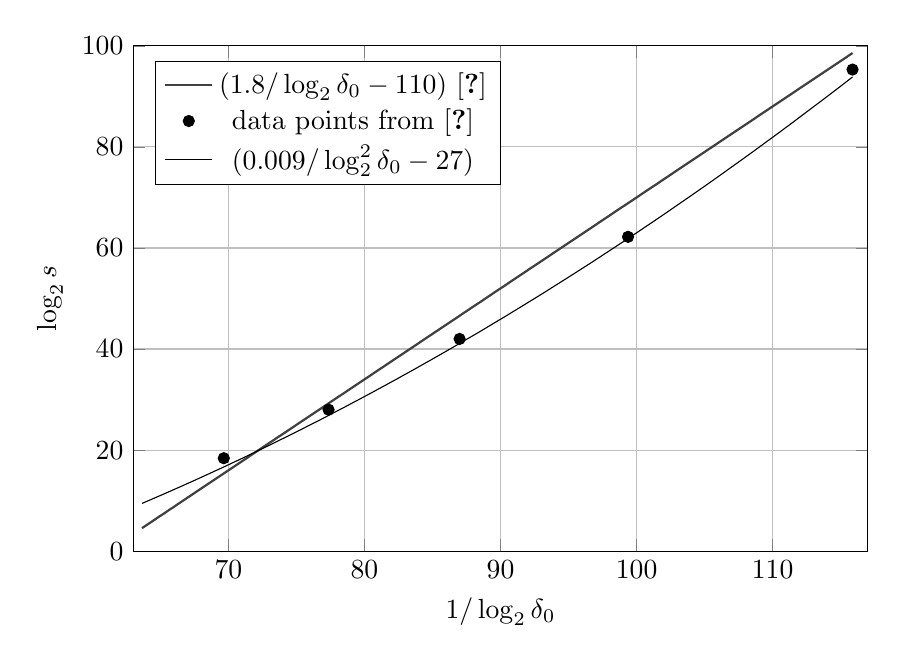
\begin{tikzpicture}[xscale=1,yscale=1]
\begin{axis}[xmin=63,xmax=117,ymin=0.0,ymax=100.0,grid=both,legend pos=north west,xlabel=$1/\log_2 \delta_0 $,ylabel=$\log_2 s$,width=0.9\textwidth,height=8cm]
\addplot[color=darkgray,thick] coordinates {
(115.87, 98.57)  (114.92, 96.85)  (113.98, 95.16)  (113.05, 93.50) 
(112.14, 91.86)  (111.25, 90.25)  (110.37, 88.67)  (109.50, 87.11) 
(108.65, 85.57)  (107.81, 84.06)  (106.98, 82.57)  (106.17, 81.11) 
(105.37, 79.66)  (104.58, 78.24)  (103.80, 76.84)  (103.03, 75.46) 
(102.28, 74.10)  (101.54, 72.76)  (100.80, 71.44)  (100.08, 70.14) 
(99.37, 68.86)  (98.66, 67.60)  (97.97, 66.35)  (97.29, 65.12)  (96.62,
63.91)  (95.95, 62.71)  (95.30, 61.54)  (94.65, 60.37)  (94.01, 59.23) 
(93.39, 58.09)  (92.77, 56.98)  (92.15, 55.88)  (91.55, 54.79)  (90.95,
53.72)  (90.37, 52.66)  (89.78, 51.61)  (89.21, 50.58)  (88.65, 49.56) 
(88.09, 48.56)  (87.53, 47.56)  (86.99, 46.58)  (86.45, 45.61)  (85.92,
44.66)  (85.39, 43.71)  (84.88, 42.78)  (84.36, 41.86)  (83.86, 40.94) 
(83.36, 40.04)  (82.86, 39.15)  (82.38, 38.28)  (81.89, 37.41)  (81.42,
36.55)  (80.94, 35.70)  (80.48, 34.86)  (80.02, 34.03)  (79.56, 33.21) 
(79.11, 32.40)  (78.67, 31.60)  (78.23, 30.81)  (77.79, 30.03)  (77.36,
29.25)  (76.94, 28.49)  (76.52, 27.73)  (76.10, 26.98)  (75.69, 26.24) 
(75.28, 25.51)  (74.88, 24.78)  (74.48, 24.06)  (74.09, 23.35)  (73.69,
22.65)  (73.31, 21.96)  (72.93, 21.27)  (72.55, 20.59)  (72.17, 19.91) 
(71.80, 19.25)  (71.44, 18.59)  (71.08, 17.94)  (70.72, 17.29)  (70.36,
16.65)  (70.01, 16.02)  (69.66, 15.39)  (69.32, 14.77)  (68.97, 14.15) 
(68.64, 13.55)  (68.30, 12.94)  (67.97, 12.35)  (67.64, 11.76)  (67.32,
11.17)  (66.99, 10.59)  (66.68, 10.02)  (66.36, 9.45)  (66.05, 8.88) 
(65.74, 8.33)  (65.43, 7.77)  (65.13, 7.23)  (64.82, 6.68)  (64.53,
6.15)  (64.23, 5.61)  (63.94, 5.09)  (63.65, 4.56) };
\addlegendentry{$(1.8/\log_2 \delta_0  - 110)$ \cite{LindnerP10}}

\addplot[only marks] coordinates {
(69.66, 18.40)  (77.36, 28.00)  (86.99, 42.00)  (99.37, 62.20)  (115.87, 95.30) 
};
\addlegendentry{data points from \cite{DBLP:conf/ctrsa/LiuN13}}

\addplot[color=black] coordinates {
(115.87, 93.83)  (114.92, 91.85)  (113.98, 89.92)  (113.05, 88.03) 
(112.14, 86.19)  (111.25, 84.39)  (110.37, 82.63)  (109.50, 80.92) 
(108.65, 79.24)  (107.81, 77.61)  (106.98, 76.01)  (106.17, 74.45) 
(105.37, 72.92)  (104.58, 71.43)  (103.80, 69.97)  (103.03, 68.55) 
(102.28, 67.15)  (101.54, 65.79)  (100.80, 64.45)  (100.08, 63.14) 
(99.37, 61.86)  (98.66, 60.61)  (97.97, 59.39)  (97.29, 58.19)  (96.62,
57.01)  (95.95, 55.86)  (95.30, 54.74)  (94.65, 53.63)  (94.01, 52.55) 
(93.39, 51.49)  (92.77, 50.45)  (92.15, 49.43)  (91.55, 48.43)  (90.95,
47.45)  (90.37, 46.49)  (89.78, 45.55)  (89.21, 44.63)  (88.65, 43.72) 
(88.09, 42.83)  (87.53, 41.96)  (86.99, 41.10)  (86.45, 40.26)  (85.92,
39.44)  (85.39, 38.63)  (84.88, 37.84)  (84.36, 37.06)  (83.86, 36.29) 
(83.36, 35.54)  (82.86, 34.80)  (82.38, 34.07)  (81.89, 33.36)  (81.42,
32.66)  (80.94, 31.97)  (80.48, 31.29)  (80.02, 30.63)  (79.56, 29.97) 
(79.11, 29.33)  (78.67, 28.70)  (78.23, 28.08)  (77.79, 27.47)  (77.36,
26.86)  (76.94, 26.27)  (76.52, 25.69)  (76.10, 25.12)  (75.69, 24.56) 
(75.28, 24.00)  (74.88, 23.46)  (74.48, 22.92)  (74.09, 22.40)  (73.69,
21.88)  (73.31, 21.37)  (72.93, 20.86)  (72.55, 20.37)  (72.17, 19.88) 
(71.80, 19.40)  (71.44, 18.93)  (71.08, 18.47)  (70.72, 18.01)  (70.36,
17.56)  (70.01, 17.11)  (69.66, 16.67)  (69.32, 16.24)  (68.97, 15.82) 
(68.64, 15.40)  (68.30, 14.99)  (67.97, 14.58)  (67.64, 14.18)  (67.32,
13.78)  (66.99, 13.39)  (66.68, 13.01)  (66.36, 12.63)  (66.05, 12.26) 
(65.74, 11.89)  (65.43, 11.53)  (65.13, 11.17)  (64.82, 10.82)  (64.53,
10.47)  (64.23, 10.13)  (63.94, 9.79)  (63.65, 9.46)};
\addlegendentry{$(0.009/\log_2^2 \delta_0 - 27)$}
\end{axis}
\end{tikzpicture}
\caption{BKZ running times in seconds $s$ for given values of $\delta_0$.}
\label{fig:delta0-to-running-time}
\end{figure}


Using this model, we can give an analogue of Table \ref{tab:concrete_Distinguishing} in which the BKZ entries are obtained using the above approximate model.

\begin{table}[!htb]
\begin{center}
\begin{tabular}{|r|r|r||r|r|r|r|r||r|r|r|r|r|} 
\hline
$n$ & $q$ & $\alpha q$ & \multicolumn{5}{|c||}{BKW} &  \multicolumn{5}{|c|}{BKZ 2.0 Simulator Model}\\
\hline
\multicolumn{3}{|c||}{ }  &   $t$   & $\log_2 m$ & $\log_2 \#\Zq$ & $\log_2 \#\Z_2$ & $\log_2 \#\Ldis$ & $\log_2 \PrS$ & $\log_2 m$ & $\log_2 \#\Zq$ & $\log_2 \#\Z_2$ & $\log_2 \#\Ldis$\\
\hline
\multicolumn{13}{|c|}{Regev \cite{regev:acm09}}\\
\hline
128 &  16411 & 11.81 & 3.2 &  81.62 &  93.84 &  97.65 &  83.85 & -14 &  22.50 &  61.90 &  65.71 &  22.50\\
256 &  65537 & 25.53 & 3.1 & 126.26 & 179.76 & 183.76 & 168.79 & -35 &  44.48 & 174.46 & 178.46 &  44.48\\
512 & 262147 & 57.06 & 3.1 & 337.92 & 350.80 & 354.97 & 338.02 & -94 & 104.47 & 518.62 & 522.79 & 104.47\\
\hline
\multicolumn{13}{|c|}{Lindner \& Peikert \cite{LindnerP10}}\\
\hline
128 &   2053 &  2.70 & 2.9 &  63.86 &  82.40 &  85.86 &  72.73 & -14 &  22.28 &  57.06 &  60.52 & 22.28\\
256 &   4099 &  3.34 & 2.8 & 105.08 & 151.45 & 155.04 & 140.64 & -33 &  42.21 & 151.16 & 154.74 & 42.21\\
512 &   4099 &  2.90 & 2.6 & 157.78 & 278.01 & 281.59 & 266.14 & -86 &  96.09 & 424.45 & 428.03 & 96.09\\
\hline
\end{tabular}
\end{center}
\caption{Cost of distinguishing LWE samples from uniform as reported as ``Distinguish'' in \cite{LindnerP10}, compared to Corollary~\ref{cor:distinguish}. BKZ estimates obtained using BKZ 2.0 simulator-derived cost estimate.}
\label{tab:concrete_Distinguishing_BKZ_2-0}
\end{table}

Thus, we can reasonably conclude that, under the assumptions made above, employing lattice reduction in a pure distinguishing approach is out-performed by BKW in surprisingly low dimension.

\subsection{Short Integer Solutions: Combinatorial}
Recall that if we consider the set of samples from $\Ldis$ used during the course of the BKW algorithm as determining a $q$-ary lattice, and the noisy vector as denoting a point close to a lattice point, we may consider the BKW algorithm as analysed in Corollary~\ref{cor:distinguish} as a combinatorial approach for sampling a sparse $\mathbf{u}$ in the dual lattice with entries $\in \{-1,0,1\}$. Hence, it is related to a combinatorial approach for finding short dual-($q$-ary)lattice vectors as briefly sketched in \cite[p. 156]{micciancio-regev:pqc2009} (cf.\ also \cite{lyubashevsky-micciancio-peikert-rosen:fse2008}). These algorithms, however, operate somewhat differently to BKW - given a relatively small set of LWE samples, these are divided into a small number of subsets. Within each subset, we compute all linear combinations of the members of that subset such that the coefficients of these linear combinations are in $\{-b',\ldots,b'\}$ (note that the parameter $b'$ is unrelated to the parameter $b$ used in this work). 

The algorithm sketched by \cite{micciancio-regev:pqc2009} uses the generalised birthday paradox to produce collisions among samples produced by inter-addition, with the parameters of the algorithm being chosen such that we expect to obtain a single short vector in the dual-lattice vector.

There are some significant differences between such algorithms and BKW, stemming from the assumption of the former that we only have access to a very small number of LWE samples. This requires the `expansion' of the sample set in such a way that when we search for collisions, we are almost certain to find enough. On the other hand, due to this expansion, the initial samples must be separated into disjoint lists. Thus, probably the easiest way to describe the algorithm in \cite{micciancio-regev:pqc2009} in terms of BKW is to imagine a variant of BKW where, if a sample is not in a given table, we add this sample plus \emph{all} $\{-b,\ldots,b\}$-bounded linear combinations of this sample with the pre-existing table entries, to the table. To give a strict analogue to \cite{micciancio-regev:pqc2009}, on finding a subsequent collision, we would need to store a list of all noise elements which had been added to a sample and ensure that, if we want to eliminate a sample, that the set of noise elements belonging to the sample and the set of noise elements belonging to the table entry are disjoint.

However, the fundamental difference stems from the assumption that the number of samples is restricted. If this is not the case (as we assume), then it is clear that BKW delivers a much shorter dual lattice vector.

\subsection{Bounded Distance Decoding: Lattice Reduction}
In \cite{LindnerP10}, the authors propose a method to solve LWE instances which consists of $q$-ary lattice reduction, then employing a decoding stage to determine the secret. The decoding stage used is essentially a straightforward modification of Babai's well-known nearest plane algorithm for CVP. The authors estimate the running-time of the BKZ algorithm in producing a basis `reduced-enough' for the decoding stage of the algorithm to succeed, then add the cost of the decoding stage.

To obtain comparable complexity results, we calculate upper bounds on the bit operation counts for two data-points based on the running times reported in \cite{LindnerP10} multiplied by the clock speed of the CPU used. As can be seen from Table \ref{tab:concrete_Lindneretal}, unsurprisingly these indicate substantially lower complexities than for BKW. In addition, the memory requirements of this approach are small compared to the memory requirements of BKW. 

\begin{table}[!htb]
\begin{center}
\begin{tabular}{|r|r|r||r|r|r|r|r||r|r|r|r|r|} 
\hline
$n$ & $q$ & $\alpha q$ & \multicolumn{5}{|c||}{BKW} &  \multicolumn{5}{|c|}{NTL-BKZ Lindner/Peikert Model}\\
\hline
\multicolumn{3}{|c||}{ }  &   $t$   & $\log_2 m$ & $\log_2 \#\Zq$ & $\log_2 \#\Z_2$ & $\log_2 \#\Ldis$ & $\log_2 \PrS$ & $\log_2 m$ & $\log_2 \#\Zq$ & $\log_2 \#\Z_2$ & $\log_2 \#\Ldis$\\
\hline
136 &   2003 & 5.19  & 2.6 & 67.49 & 93.77 & 97.23 & 84.15 & -25 & 33.46 & 91.35 & 94.81 & 33.46\\
214 &  16381 & 2.94  & 3.4 & 76.90 & 128.36 & 132.16 & 117.54 & -18 & 26.95 & 82.31 & 86.11 & 26.95\\
\hline
\end{tabular}
\end{center}
\caption{Cost of solving Search-LWE reported as ``Decode'' in \cite{LindnerP10}, compared to the cost solving Decision-LWE with BKW}
\label{tab:concrete_Lindneretal}
\end{table}

\subsection{Bounded Distance Decoding: Combinatorial}
We can take the approach of viewing LWE as being the problem of solving BDD in a random $q$-ary lattice with a random target $\mathbf{t}=\mathbf{A}\mathbf{s}+\mathbf{e}$. To solve the LWE problem formulated thus, we have several choices of lattice-based algorithms. However, for several such algorithms, tight complexity estimates are unavailable, thus making comparison to BKW loose. One algorithm for which more precise complexity estimates are available is the AKS (Ajtai, Kumar \& Sivakumar) algorithm for solving the shortest vector problem \cite{ajtai-kumar-sivakumar:ccc2002}. This algorithm is notable as being the first proposed singly-exponential SVP algorithm.

It is beyond the scope of this paper to give details of the AKS algorithm -- we are interested solely in the complexity. In the original paper by Ajtai, Kumar \& Sivakumar, no explicit running-time bound was given. Subsequent developments of the AKS algorithm by Regev, Nguyen and Vidick, Micciancio and Voulgaris, Pujol and Stehle delivered algorithms which were of time complexity $2^{16n+o(n)}$, $2^{5.9n+o(n)}$, $2^{3.4n+o(n)}$ and $2^{2.7n+o(n)}$, respectively \cite{DBLP:conf/codcry/HanrotPS11}.